\documentclass[../../InformazioneQuantistica.tex]{subfiles}

\begin{document}

\section{Qubit}
\lesson{2}{28/2/2019}
\textbf{Riepilogando}, abbiamo sostituito lo \textit{stato classico} di un bit con uno \textit{stato quantistico}, dato da un \textbf{qubit}\index{Qubit}, costituito da una combinazione lineare di due stati fondamentali $\ket{0}$ e $\ket{1}$:
\begin{align*}
\ket{\psi} = \cos\frac{\theta}{2} \ket{0} + e^{i\varphi} \sin\frac{\theta}{2}\ket{1}
\end{align*}


\begin{figure}[H]
\centering


\tikzset{every picture/.style={line width=0.75pt}} %set default line width to 0.75pt        
\begin{center}
\begin{tikzpicture}[x=0.75pt,y=0.75pt,yscale=-1,xscale=1]
%uncomment if require: \path (0,300); %set diagram left start at 0, and has height of 300

%Straight Lines [id:da35494731744920616] 
\draw    (180.08,120.33) -- (270.58,120.33) ;


%Straight Lines [id:da8080577379615441] 
\draw    (180.5,160) -- (270.25,160) ;



% Text Node
\draw (286,118.5) node   {$|0\rangle $};
% Text Node
\draw (285.5,159) node   {$|1\rangle $};


\end{tikzpicture}
\end{center}
\caption{Come nel caso classico, rappresentiamo i \textit{qubit} come linee, che saranno opportunamente collegate agli input delle porte logiche\label{fig:qubit-righe}}
\end{figure}


Ricordiamo che $\ket{\psi}$ e $e^{i\alpha}\ket{\psi}$ rappresentano lo stesso stato, dato che gli stati in \MQ sono definiti da \textit{raggi vettori} definiti a meno di una fase globale.\\

Ci chiediamo: quanta \textit{informazione}\marginpar{Informazione in un qubit} (in senso classico) racchiude un qubit? Abbiamo due possibili risposte, in contraddizione tra di loro:
\begin{itemize}
\item Un qubit è l'analogo quantistico del bit, e quindi racchiude la \textit{stessa quantità di informazione}
\item Un qubit è univocamente definito da \textbf{due numeri complessi}, o da due angoli $\theta$, $\varphi$, che hanno \q{infinite cifre} e quindi possono codificare \textit{infinita informazione}. Per esempio potremmo scegliere (in \si{\radian}) $\theta=0.10010\dots$ e codificare nelle infinite cifre decimali un qualsiasi messaggio in binario.
\end{itemize}
In realtà, in pratica per produrre un output dovremo effettuare una \textbf{misura} sul qubit, che avrà due soli possibili risultati: $\ket{0}$ o $\ket{1}$. L'informazione sullo stato può essere ricavata solo da un grande insieme di qubit perfettamente identici, sui quali possiamo fare tante misure e, con tecniche di \textit{tomografia quantistica}, ricostruire, almeno in principio, gli esatti coefficienti della $\ket{\psi}$ originaria. In particolare l'informazione estratta sarà proporzionale al numero di misure effettuate, ritornando così ad un caso equivalente ad un sistema classico di \textit{molti bit}.\\

Vi è comunque un vantaggio a tutto ciò: i \textit{numeri complessi} che definiscono la $\ket{\psi}$ sono \textbf{disponibili durante il processo quantistico}, cioè prima della misura, e quindi possono essere usati per la sua evoluzione. In altre parole, \textit{computazionalmente} è \q{come se avessimo più informazione disponibile}, anche se, alla fine, siamo costretti a scartarne la maggior parte, estraendo un risultato \q{condensato}.\\

Un \textbf{computer quantistico}\index{Computer!quantistico} si basa allora sull'inizializzare opportunamente un certo numero di qubit, che poi si evolvono in modo unitario attraverso opportune porte logiche.

\begin{figure}[H]
\centering


\tikzset{every picture/.style={line width=0.75pt}} %set default line width to 0.75pt        
\begin{center}
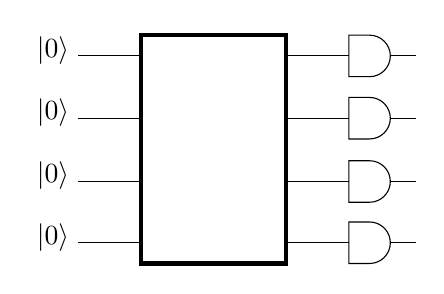
\begin{tikzpicture}[x=0.75pt,y=0.75pt,yscale=-1,xscale=1]
%uncomment if require: \path (0,300); %set diagram left start at 0, and has height of 300

%Straight Lines [id:da6516338805729034] 
\draw    (220,160) -- (250.25,160) ;


%Straight Lines [id:da3483397623450477] 
\draw    (220,130.5) -- (250.25,130.5) ;


%Straight Lines [id:da9238618827802416] 
\draw    (220,100) -- (250.25,100) ;


%Straight Lines [id:da17017205003570535] 
\draw    (220,70) -- (250.25,70) ;


%Shape: Rectangle [id:dp990517862527216] 
\draw  [line width=1.5]  (250.25,60) -- (320.25,60) -- (320.25,170) -- (250.25,170) -- cycle ;
%Straight Lines [id:da283851976727008] 
\draw    (320.5,160) -- (350.75,160) ;


%Straight Lines [id:da3154319354667985] 
\draw    (320.5,130.5) -- (350.75,130.5) ;


%Straight Lines [id:da6302150655412055] 
\draw    (320.5,100) -- (350.75,100) ;


%Straight Lines [id:da3354735688576296] 
\draw    (320.5,70) -- (350.75,70) ;


%Flowchart: Delay [id:dp8725812367609944] 
\draw   (350.5,150) -- (360.5,150) .. controls (366.02,150) and (370.5,154.48) .. (370.5,160) .. controls (370.5,165.52) and (366.02,170) .. (360.5,170) -- (350.5,170) -- cycle ;
%Flowchart: Delay [id:dp5735117515253538] 
\draw   (350.5,120.5) -- (360.5,120.5) .. controls (366.02,120.5) and (370.5,124.98) .. (370.5,130.5) .. controls (370.5,136.02) and (366.02,140.5) .. (360.5,140.5) -- (350.5,140.5) -- cycle ;
%Flowchart: Delay [id:dp8647107846726951] 
\draw   (350.5,90) -- (360.5,90) .. controls (366.02,90) and (370.5,94.48) .. (370.5,100) .. controls (370.5,105.52) and (366.02,110) .. (360.5,110) -- (350.5,110) -- cycle ;
%Flowchart: Delay [id:dp9147779152625295] 
\draw   (350.5,60) -- (360.5,60) .. controls (366.02,60) and (370.5,64.48) .. (370.5,70) .. controls (370.5,75.52) and (366.02,80) .. (360.5,80) -- (350.5,80) -- cycle ;
%Straight Lines [id:da8078837867724449] 
\draw    (370.5,70) -- (382.75,70) ;


%Straight Lines [id:da04251360456824571] 
\draw    (370.5,100) -- (382.75,100) ;


%Straight Lines [id:da30533401825899187] 
\draw    (370.5,130.5) -- (382.75,130.5) ;


%Straight Lines [id:da6881317452621902] 
\draw    (370.5,160) -- (382.75,160) ;



% Text Node
\draw (208,67.5) node   {$|0\rangle $};
% Text Node
\draw (208,97.5) node   {$|0\rangle $};
% Text Node
\draw (208,127.5) node   {$|0\rangle $};
% Text Node
\draw (208,157.5) node   {$|0\rangle $};


\end{tikzpicture}
\end{center}
\caption{Schema di un computer quantistico, dove l'input consiste in $4$ qubit inizializzati a $\ket{0}$\label{fig:computer-quantico}}
\end{figure}

Ad un certo istante dell'evoluzione, il computer quantistico si trova in un generico stato $\ket{\psi}$, che consiste nello stato di $n$ qubit, dato da una delle possibili combinazioni lineari (con coefficienti $\Psi_{\vec{\alpha}}$) dei prodotti tensori degli stati $\ket{\alpha_i}=\{\ket{0},\ket{1}\}$ dei singoli qubit:
\begin{align*}
\ket{\psi} &=\sum_{\vec{\alpha}} \Psi_{\alpha_1,\alpha_2,\dots,\alpha_N}\left( \bigotimes_{i=1}^N \ket{\alpha_i} = \ket{\alpha_1}\ket{\alpha_2}\dots\ket{\alpha_N} \right)=\\
&\equiv\sum_{\vec{\alpha}} \Psi_{\alpha_1, \dots, \alpha_N} \ket{\alpha_1, \dots, \alpha_N}
\end{align*}
dove i coefficienti $\Psi_{\vec{\alpha}} \in \bb{C}$ sono opportunamente normalizzati:
\begin{align*}
\sum_{\vec{\alpha}} \left| \Psi_{\vec{\alpha}}\right|^2 = 1
\end{align*}

\textbf{Nota}: in informazione quantistica supponiamo sempre di avere a che fare con qubit che sono \textbf{distinguibili} tra loro, e quindi non avremo problemi di statistica fermionica/bosonica (che comunque iniziano a essere esplorati da alcuni studi attuali).\\

Nella pratica non è per nulla semplice poter realizzare questi stati. $\ket{0}$ e $\ket{1}$ di un singolo qubit sono in genere separati da una piccolissima quantità di energia, che può essere fornita dal bagno termico in cui si trova il sistema. In altre parole, effetti termici possono modificare lo stato di input, rendendolo inutilizzabile. Ecco perché i computer quantistici sono realizzati in sistemi controllati tramite avanzate tecniche criogeniche.\\

Analogamente al caso classico,\marginpar{Ogni operatore è la composizione di porte logiche} si può dimostrare che \textbf{un qualsiasi operatore quantistico} $O$ che agisce su $n$ qubit può essere\textbf{ scomposto} come l'azione combinata di opportune \textbf{porte logiche quantistiche fondamentali}. In genere, trovare tale combinazione non è però un problema banale - spesso si hanno solo risultati di esistenza, o bound sul numero di gate necessari.

\begin{figure}[H]
\centering


\tikzset{every picture/.style={line width=0.75pt}} %set default line width to 0.75pt        
\begin{center}
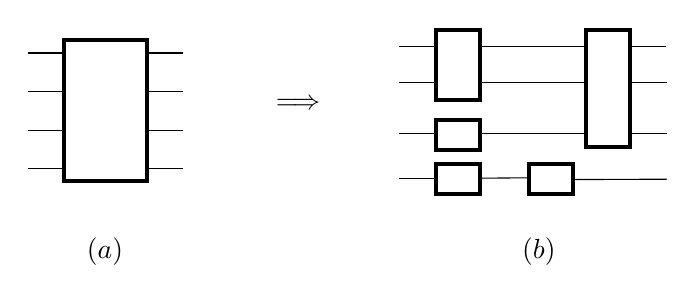
\begin{tikzpicture}[x=0.75pt,y=0.75pt,yscale=-1,xscale=1]
%uncomment if require: \path (0,300); %set diagram left start at 0, and has height of 300

%Straight Lines [id:da5358850368993795] 
\draw    (143,142.82) -- (160.24,142.82) ;


%Straight Lines [id:da6806658389070328] 
\draw    (143,124.58) -- (160.24,124.58) ;


%Straight Lines [id:da8151023000430018] 
\draw    (143,105.73) -- (160.24,105.73) ;


%Straight Lines [id:da852801527417671] 
\draw    (143,87.18) -- (160.24,87.18) ;


%Shape: Rectangle [id:dp5049680819457896] 
\draw  [line width=1.5]  (160.24,81) -- (200.12,81) -- (200.12,149) -- (160.24,149) -- cycle ;
%Straight Lines [id:da3257969992027685] 
\draw    (200.26,142.82) -- (217.5,142.82) ;


%Straight Lines [id:da6006292828733499] 
\draw    (200.26,124.58) -- (217.5,124.58) ;


%Straight Lines [id:da575866078063267] 
\draw    (200.26,105.73) -- (217.5,105.73) ;


%Straight Lines [id:da3668795795454598] 
\draw    (200.26,87.18) -- (217.5,87.18) ;


%Shape: Rectangle [id:dp07164813109342494] 
\draw  [line width=1.5]  (339.57,76) -- (360.83,76) -- (360.83,110) -- (339.57,110) -- cycle ;
%Straight Lines [id:da5550547061584261] 
\draw    (321.6,84.18) -- (338.83,84.18) ;


%Straight Lines [id:da7030246183368658] 
\draw    (321.6,101.52) -- (338.83,101.52) ;


%Straight Lines [id:da014046487694113319] 
\draw    (361.6,84.18) -- (410.67,84.18) ;


%Straight Lines [id:da7902809542944893] 
\draw    (361.6,101.52) -- (410.67,101.52) ;


%Shape: Rectangle [id:dp1720031992227251] 
\draw  [line width=1.5]  (411.57,76) -- (432.83,76) -- (432.83,132.67) -- (411.57,132.67) -- cycle ;
%Shape: Rectangle [id:dp3123232058600962] 
\draw  [line width=1.5]  (339.57,119.33) -- (360.83,119.33) -- (360.83,134) -- (339.57,134) -- cycle ;
%Straight Lines [id:da9070147074432569] 
\draw    (321.6,126.18) -- (338.83,126.18) ;


%Straight Lines [id:da017645574926253182] 
\draw    (361.6,126.18) -- (410.67,126.18) ;


%Shape: Rectangle [id:dp0003927881970808844] 
\draw  [line width=1.5]  (339.57,140.67) -- (360.83,140.67) -- (360.83,155.33) -- (339.57,155.33) -- cycle ;
%Straight Lines [id:da11231237711041464] 
\draw    (321.6,147.52) -- (338.83,147.52) ;


%Straight Lines [id:da28491338313190284] 
\draw    (360.93,147.52) -- (383.33,147.33) ;


%Shape: Rectangle [id:dp5206294486499532] 
\draw  [line width=1.5]  (384.24,140.67) -- (405.5,140.67) -- (405.5,155.33) -- (384.24,155.33) -- cycle ;
%Straight Lines [id:da8125060984498069] 
\draw    (405.6,148.18) -- (450.67,148) ;


%Straight Lines [id:da2769560169405245] 
\draw    (433.6,126.18) -- (450.83,126.18) ;


%Straight Lines [id:da5586286524840975] 
\draw    (433.6,101.52) -- (450.83,101.52) ;


%Straight Lines [id:da43666666448278724] 
\draw    (432.93,84.18) -- (450.17,84.18) ;



% Text Node
\draw (273,112) node   {$\Longrightarrow $};
% Text Node
\draw (180,183) node   {$( a)$};
% Text Node
\draw (389,183) node   {$( b)$};


\end{tikzpicture}
\end{center}
\caption{Un qualsiasi operatore $O$ (a) che esegue una certa operazione su $n$ qubit può essere scomposto in  una serie di porte logiche fondamentali (b) opportunamente collegate che svolgono la medesima operazione.\label{fig:scomposizione-porte-logiche}}
\end{figure}

\section{Porte logiche quantistiche}
Nella seguente sezione ci occuperemo di esaminare le principali porte logiche utilizzate in computazione quantistica.

\subsection{Porte a 1 qubit}
Le porte a $1$ qubit sono rappresentate da matrici unitarie $2\times 2$, di solito espresse nella \textbf{base computazionale} $\{\ket{0}, \ket{1}\}$.\index{Base computazionale!1 qubit} Nella notazione matriciale ricordiamo che:
\begin{align*}
\ket{0} = \begin{pmatrix} 1 \\ 0 \end{pmatrix} \qquad \ket{1} = \begin{pmatrix} 0 \\ 1 \end{pmatrix}
\end{align*}

Un primo esempio è dato dalla \textbf{porta di Hadamard}\marginpar{Porta di Hadamard}\index{Porte logiche!Hadamard}, la cui rappresentazione matriciale è data da:
\begin{align*}
H = \frac{1}{\sqrt{2}} \begin{pmatrix}
1 & 1\\1 & -1
\end{pmatrix}
\end{align*}
e il cui elemento circuitale è rappresentato come:



\tikzset{every picture/.style={line width=0.75pt}} %set default line width to 0.75pt        
\begin{center}
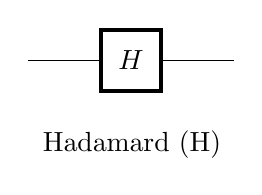
\begin{tikzpicture}[x=0.75pt,y=0.75pt,yscale=-1,xscale=1]
%uncomment if require: \path (0,300); %set diagram left start at 0, and has height of 300

%Straight Lines [id:da01764244060439424] 
\draw    (180.67,140.33) -- (279.67,140.33) ;


%Shape: Rectangle [id:dp07818144394667903] 
\draw  [fill={rgb, 255:red, 255; green, 255; blue, 255 }  ,fill opacity=1 ][line width=1.5]  (215.62,125.5) -- (244.71,125.5) -- (244.71,155.17) -- (215.62,155.17) -- cycle ;

% Text Node
\draw (230.67,180.67) node  [align=left] {Hadamard (H)};
% Text Node
\draw (230.17,140.33) node   {$H$};


\end{tikzpicture}
\end{center}

Facendola agire sugli stati della base, tramite un \textit{prodotto di matrice per vettore}, otteniamo la sua \textit{tavola di verità}:
\begin{align*}
H \ket{0} &= \frac{1}{\sqrt{2}} (\ket{0} + \ket{1}) = \ket{+}_x\\
H \ket{1} &= \frac{1}{\sqrt{2}} (\ket{0} - \ket{1}) = \ket{-}_x
\end{align*} 
L'azione di $H$ può essere schematizzata come un passaggio dalla base degli autostati dell'operatore $\sigma_z$ (che possiamo far coincidere con i $\ket{0}$ e $\ket{1}$ della base computazionale) a quella dell'operatore $\sigma_x$ $\{\ket{+},\ket{-}\}$ (l'equivalente di una \textit{rotazione}, se fossimo nel comune spazio cartesiano in $d=3$)\footnote{Qui le $\sigma_i$ indicano le \textbf{matrici di Pauli}.}.\\

Una porta quantistica \textit{senza analogo classico} è quella che \q{aggiunge una fase relativa}, detta di \textbf{phase-shift}:\marginpar{Operatore phase-shift}\index{Porte logiche!Phase-shift}
\begin{align*}
R_z(\delta) = \begin{pmatrix}
1 & 0\\0 & e^{i\delta}
\end{pmatrix}
\end{align*}
che agisce come:
\begin{align*}
R_z(\delta) \ket{\psi} = \cos\frac{\theta}{2} \ket{0} + e^{i(\varphi + \delta)} \sin\frac{\theta}{2} \ket{1}
\end{align*}
ed è rappresentata nei circuiti mediante il simbolo:



\tikzset{every picture/.style={line width=0.75pt}} %set default line width to 0.75pt        
\begin{center}
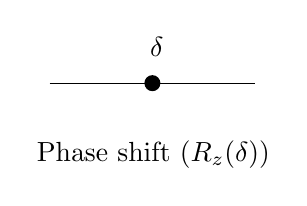
\begin{tikzpicture}[x=0.75pt,y=0.75pt,yscale=-1,xscale=1]
%uncomment if require: \path (0,300); %set diagram left start at 0, and has height of 300

%Straight Lines [id:da9921299484654684] 
\draw    (160.67,120.33) -- (259.67,120.33) ;


%Straight Lines [id:da4318238438195179] 
\draw    (210.17,120.33) ;

\draw [shift={(210.17,120.33)}, rotate = 0] [color={rgb, 255:red, 0; green, 0; blue, 0 }  ][fill={rgb, 255:red, 0; green, 0; blue, 0 }  ][line width=0.75]      (0, 0) circle [x radius= 3.35, y radius= 3.35]   ;

% Text Node
\draw (212.33,102.67) node   {$\delta $};
% Text Node
\draw (210.67,154.67) node  [align=left] {Phase shift ($\displaystyle R_{z}( \delta )$)};


\end{tikzpicture}
\end{center}

Si dimostra, come verificheremo più avanti, che un generico stato $\ket{\psi}$ di un singolo qubit può essere ottenuto partendo da $\ket{0}$ applicando una successione di porte logiche a $1$-bit:
\begin{align*}
\ket{\psi} = R_z\left(\frac{\pi}{2} + \varphi\right) H R_z(\theta) H \ket{0}
\end{align*}

\subsection{Porte a 2 qubit}
Un generico stato di $2$ qubit è una combinazione di $4$ possibili stati (in generale, $n$ qubit sono combinazioni di $2^n$ possibilità):
\begin{align*}
\ket{\psi} = \alpha_{00}\ket{00} + \alpha_{01}\ket{01} + \alpha_{10}\ket{10} + \alpha_{11} \ket{11}
\end{align*}
con la normalizzazione:
\begin{align*}
\sum_{n=0}^3 |\alpha_n|^2 = 1 \qquad \alpha_{n} \in \bb{C}
\end{align*}
dove $n$ va da $0$ a $3$ e \q{codifica} le $4$ possibilità dei due indici binari ($0=00$, $1=01$, $2=10$, $3=11$). Useremo spesso questa \q{notazione mista} poiché la forma in \textbf{binario} è utile per riconoscere immediatamente a quale autoket si riferisca un certo coefficiente, mentre quella \textbf{decimale} è comoda per gli indici delle sommatorie.\\

La \textbf{base computazionale}\index{Base computazionale!2 qubit} $\{\ket{00}, \ket{01}, \ket{10}, \ket{11}\}$, in notazione matriciale, è data da:
\begin{align*}
\ket{00} = \begin{pmatrix}1 \\ 0 \\ 0 \\ 0 \end{pmatrix} \quad
\ket{01} = \begin{pmatrix}0 \\ 1 \\ 0 \\ 0 \end{pmatrix} \quad
\ket{10} = \begin{pmatrix}0 \\ 0 \\ 1 \\ 0 \end{pmatrix} \quad
\ket{11} = \begin{pmatrix}0 \\ 0 \\ 0 \\ 1 \end{pmatrix}
\end{align*}

La prima porta logica che analizziamo è detta \textbf{CNOT}\index{Porte logiche!CNOT} (\textit{controlled not}) \marginpar{Gate CNOT} e corrisponde ad un'operazione su un bit \textit{condizionata} da un altro bit. In particolare CNOT esegue un'operazione NOT sul secondo qubit solo se il primo è pari a $1$, e non fa nulla altrimenti (ossia funge da \q{buffer} se il primo bit è $0$). Si tratta di un'operazione di not \q{controllata}, dato che viene \q{accesa} solo se il bit di controllo è pari a $1$. In notazione matriciale, usando la base $\{\ket{00}, \ket{01}, \ket{10}, \ket{11}\}$ vista sopra, è data da:
\begin{align*}
\op{CNOT} =
\left(
        \begin{array}{cc|cc}
        1 & 0 & 0 & 0 \\
        0 & 1 & 0 & 0 \\
        \hline
        0 & 0 & 0 & 1 \\
        0 & 0 & 1 & 0 \\        
        \end{array}
\right)
\end{align*}
In questa notazione, le prime due colonne (a sinistra) descrivono il funzionamento quando il bit di controllo - che è quello \textit{più significativo} nella notazione binaria, ossia quello più a sinistra - è $0$, e le ultime due quando è $1$. Perciò gli stati $\ket{\bm{0}0}$ e $\ket{\bm{0}1}$, dove tale bit di controllo è nullo, vengono mandati in se stessi senza variazioni, mentre per $\ket{\bm{1}0}$ e $\ket{\bm{1}1}$ il risultato si ottiene \textit{invertendo} il secondo bit (quello \textit{meno significativo} nella notazione binaria). Possiamo schematizzare il comportamento usando un analogo delle tavole di verità classiche (tabella \ref{tab:C-NOT}), ricordando però che lo stato iniziale (con bit di controllo indicato con $c$ e secondo bit con $a$) può essere una \textit{combinazione lineare} degli stati possibili di $2$ qubit, e di conseguenza l'output sarà anch'esso una combinazione lineare. In altre parole, in una tavola di verità quantistica è possibile che \q{più righe siano applicate contemporaneamente}.

\begin{table}[H]
\centering
\begin{tabular}{@{}llll@{}}
\toprule
$\bm{c}$ & $\bm{a}$ & $\bm{\bar{a}}$ & \textbf{out} \\ \midrule
$\ket{0}$ & $\hlc{Yellow}{\ket{0}}$ & $\ket{1}$ & $\ket{0}\hlc{Yellow}{\ket{0}}$ \\
$\ket{0}$ & $\hlc{Yellow}{\ket{1}}$ & $\ket{0}$ & $\ket{0}\hlc{Yellow}{\ket{1}}$ \\
$\ket{1}$ & $\ket{0}$ & $\hlc{SkyBlue}{\ket{1}}$ & $\ket{1}\hlc{SkyBlue}{\ket{1}}$ \\
$\ket{1}$ & $\ket{1}$ & $\hlc{SkyBlue}{\ket{0}}$ & $\ket{1}\hlc{SkyBlue}{\ket{0}}$ \\ \bottomrule
\end{tabular}
\caption{Tavola di verità per il gate CNOT}
\label{tab:C-NOT}
\end{table}

\textbf{Nota}: come si nota dalla tavola di verità la porta CNOT ha $2$ output: uno è quello condizionale descritto, e l'altro è sempre pari al qubit $c$ di controllo. In particolare, non è possibile realizzare una porta quantistica a $2$ bit con meno di $2$ output, dato che in tal caso non si potrebbe avere corrispondenza biunivoca tra stati finali e iniziali, violando l'unitarietà dell'evoluzione quantistica (torneremo su questa \textit{reversibilità} nei prossimi paragrafi).\\

Nei circuiti il gate CNOT ha la seguente rappresentazione:



\tikzset{every picture/.style={line width=0.75pt}} %set default line width to 0.75pt        
\begin{center}
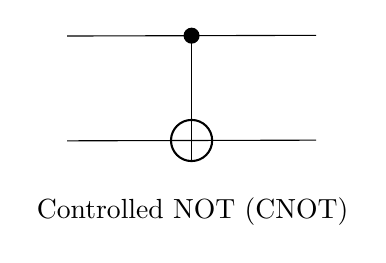
\begin{tikzpicture}[x=0.75pt,y=0.75pt,yscale=-1,xscale=1]
%uncomment if require: \path (0,300); %set diagram left start at 0, and has height of 300

%Straight Lines [id:da37432740726373037] 
\draw    (190,100) -- (310,99.67) ;


%Straight Lines [id:da2228128852300788] 
\draw    (250,99.83) -- (250,150.33) ;

\draw [shift={(250,99.83)}, rotate = 90] [color={rgb, 255:red, 0; green, 0; blue, 0 }  ][fill={rgb, 255:red, 0; green, 0; blue, 0 }  ][line width=0.75]      (0, 0) circle [x radius= 3.35, y radius= 3.35]   ;
%Shape: Circle [id:dp7117673469492589] 
\draw  [line width=0.75]  (240.08,150.33) .. controls (240.08,144.86) and (244.52,140.42) .. (250,140.42) .. controls (255.48,140.42) and (259.92,144.86) .. (259.92,150.33) .. controls (259.92,155.81) and (255.48,160.25) .. (250,160.25) .. controls (244.52,160.25) and (240.08,155.81) .. (240.08,150.33) -- cycle ;
%Straight Lines [id:da026806271903653256] 
\draw    (250,150.33) -- (250,160.25) ;


%Straight Lines [id:da8771832857323554] 
\draw    (190,150.5) -- (310,150.17) ;



% Text Node
\draw (250.5,184.5) node  [align=left] {Controlled NOT (CNOT)};


\end{tikzpicture}
\end{center}

Poiché il primo qubit in generale sarà una combinazione lineare di $\ket{0}$ e $\ket{1}$, la CNOT crea una \textit{correlazione} tra i due bit, portando alla generazione di \textbf{stati entangled}, ossia stati che non sono rappresentabili come un prodotto tensore \q{puro}:\marginpar{Stato entangled}
\begin{align*}
\ket{\psi} \neq \ket{\phi_1} \otimes \ket{\phi_2}
\end{align*}
Questo succede poiché uno stato generale è una combinazione lineare degli stati realizzati dai prodotti tensori, e solo alcune combinazioni sono anche \textit{fattorizzabili}.\\


Vediamo esplicitamente come la CNOT possa creare stati entangled.\marginpar{La CNOT può creare stati entangled} Partiamo da uno stato iniziale dato da:
\begin{align*}
\ket{\psi_i} = \left(\alpha\ket{0} + \beta\ket{1}\right) \otimes \ket{0}
\end{align*}
In cui il primo qubit (che è quello \q{di controllo}) è una combinazione di $\ket{0}$ e $\ket{1}$, ossia ha una probabilità $|\alpha|^2$ di essere $\ket{0}$ e $|\beta|^2$ di essere $\ket{1}$. Ciò si traduce in una certa probabilità che il qubit $a$ sia \textit{negato}, e in un'altra che invece non sia modificato - fino a che non si effettua una misura, i due percorsi sono \textit{entrambi realizzati}. Infatti, operando su $\ket{\psi_i}$ con CNOT otteniamo:
\begin{align*}
\op{CNOT}(\ket{\psi}_i) &\underset{(a)}{=} \op{CNOT}(\alpha \ket{00} + \beta \ket{10}) \underset{(b)}{=} \op{CNOT}(\alpha \ket{00}) + \op{CNOT}(\beta \ket{10}) =\\
&= \alpha \ket{00} + \beta \ket{11}
\end{align*}
dove in (a) abbiamo distribuito il prodotto tensore, e in (b) abbiamo usato la linearità di CNOT (dato che è un operatore unitario, e quindi lineare - infatti  ha una rappresentazione matriciale).\\
Lo stato finale è quindi \textbf{entangled}, dato che è \textbf{combinazione} di prodotti tensori, e non può essere scritto come \textbf{un solo} prodotto tensore \q{puro}. Si ha quindi una \textit{correlazione} tra due parti diverse del sistema - ciò sarà fondamentale per la computazione quantistica, dato che permette di sfruttare la maggiore libertà dell'\textit{entanglement}, un fenomeno senza analogo classico.\\

Un altro gate importante è l'analogo di CNOT per le fasi, che effettua una \textit{rotazione} di un qubit (introducendo su di esso una fase relativa) a seconda \marginpar{Gate C-PHASE}\index{Porte logiche!CPHASE} del valore di un altro qubit. Tale gate è detto \textbf{C-PHASE} (\textit{controlled phase}), e ha rappresentazione matriciale:
\begin{align*}
\op{CPHASE} =
\left(
        \begin{array}{cc|cc}
        1 & 0 & 0 & 0 \\
        0 & 1 & 0 & 0 \\
        \hline
        0 & 0 & 1 & 0 \\
        0 & 0 & 0 & e^{i\delta} \\        
        \end{array}
\right)=
\begin{pmatrix}
\bb{I}_2 & \bb{O}_2\\
\bb{O}_2 & R_z(\delta)
\end{pmatrix}
\end{align*}
Analogamente al caso di CNOT, quando il bit di controllo $c$ è $1$ allora viene applicata una $R_z(\delta)$ all'altro bit $a$, e altrimenti non si fa nulla, come mostrato nella \textit{tavola di verità} in tabella \ref{tab:C-PHASE}.

\begin{table}[H]
\centering
\begin{tabular}{@{}lll@{}}
\toprule
$\bm{c}$ & $\bm{a}$ & \textbf{out} \\ \midrule
$\ket{0}$ & $\hlc{Yellow}{\ket{0}}$ & $\ket{0}\hlc{Yellow}{\ket{0}}$ \\
$\ket{0}$ & $\hlc{Yellow}{\ket{1}}$ & $\ket{0}\hlc{Yellow}{\ket{1}}$ \\
$\ket{1}$ & $\ket{0}$ & $\ket{1}\hlc{SkyBlue}{R_z(\delta)\ket{1}}$ \\
$\ket{1}$ & $\ket{1}$ & $\ket{1}\hlc{SkyBlue}{R_z(\delta)\ket{0}}$ \\ \bottomrule
\end{tabular}
\caption{Tavola di verità per la porta CPHASE}
\label{tab:C-PHASE}
\end{table}

La rappresentazione circuitale per il gate CPHASE è la seguente:


\tikzset{every picture/.style={line width=0.75pt}} %set default line width to 0.75pt        
\begin{center}
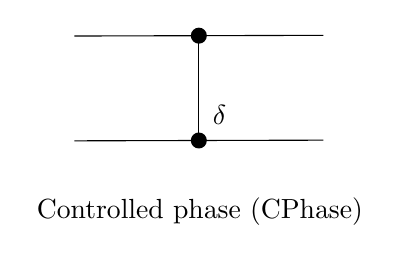
\begin{tikzpicture}[x=0.75pt,y=0.75pt,yscale=-1,xscale=1]
%uncomment if require: \path (0,300); %set diagram left start at 0, and has height of 300

%Straight Lines [id:da35716274170149065] 
\draw    (210,120) -- (330,119.67) ;


%Straight Lines [id:da753407793570797] 
\draw    (270,119.83) -- (270,170.33) ;
\draw [shift={(270,170.33)}, rotate = 90] [color={rgb, 255:red, 0; green, 0; blue, 0 }  ][fill={rgb, 255:red, 0; green, 0; blue, 0 }  ][line width=0.75]      (0, 0) circle [x radius= 3.35, y radius= 3.35]   ;
\draw [shift={(270,119.83)}, rotate = 90] [color={rgb, 255:red, 0; green, 0; blue, 0 }  ][fill={rgb, 255:red, 0; green, 0; blue, 0 }  ][line width=0.75]      (0, 0) circle [x radius= 3.35, y radius= 3.35]   ;
%Straight Lines [id:da2166973271793493] 
\draw    (210,170.5) -- (330,170.17) ;



% Text Node
\draw (270.5,204.5) node  [align=left] {Controlled phase (CPhase)};
% Text Node
\draw (280,158) node   {$\delta $};


\end{tikzpicture}
\end{center}

\subsection{Funzioni di qubit}
Occupiamoci ora di rappresentare una funzione binaria, del tipo generico:
\begin{align*}
f: \{0,1\}^n \to \{0,1\}
\end{align*}
Il problema è che, in generale, le $f(x)$ \textbf{non sono biunivoche}, e quindi\marginpar{Computazione quantistica è reversibile} non possono essere rappresentate da una serie di operazioni unitarie, in cui dallo stato finale si può recuperare l'informazione sullo stato iniziale in modo \textit{univoco}.\\
Per risolvere la situazione dobbiamo estendere tali generiche funzioni a una classe di \textbf{funzioni reversibili}. Il modo più semplice per farlo è \q{portarsi dietro l'input}, raddoppiando il numero di gradi di libertà $n$. Avremo quindi un circuito che in input ha un registro di $n$-qubit contenente lo stato iniziale $\ket{x}$, e uno di pari dimensioni (altri $n$ qubit) che contiene $\ket{0}$. L'output sarà allora $\ket{x}$ per i primi $n$ qubit (ossia di nuovo l'input) e per gli ultimi $\ket{f(x)}$. Si ha quindi un circuito che, tenendo costante il primo l'input, modifica il secondo tramite opportune funzioni.\\
In realtà lo schema si può generalizzare, partendo per il secondo registro da un generico $\ket{y}$, che si fa evolvere a $\ket{f(x) + y}$ (figura \ref{fig:computazione-reversibile}).

\begin{figure}[H]
\centering


\tikzset{every picture/.style={line width=0.75pt}} %set default line width to 0.75pt        
\begin{center}
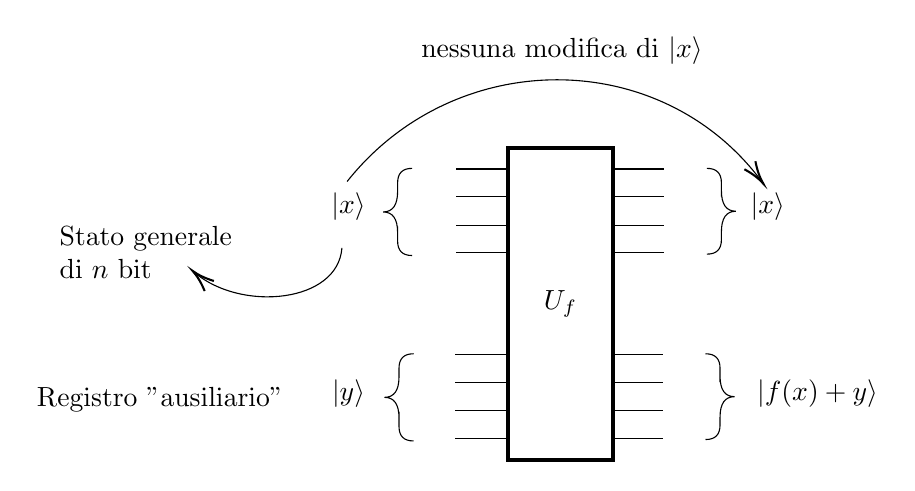
\begin{tikzpicture}[x=0.75pt,y=0.75pt,yscale=-1,xscale=1]
%uncomment if require: \path (0,300); %set diagram left start at 0, and has height of 300

%Straight Lines [id:da8018762189626685] 
\draw    (240.67,130.33) -- (265.46,130.33) ;


%Straight Lines [id:da9959980995216082] 
\draw    (240.67,117.11) -- (265.46,117.11) ;


%Straight Lines [id:da7944941960941587] 
\draw    (240.67,103.44) -- (265.46,103.44) ;


%Straight Lines [id:da634487408707328] 
\draw    (240.67,90) -- (265.46,90) ;


%Shape: Rectangle [id:dp021998310168785284] 
\draw  [line width=1.5]  (265.46,80) -- (316.2,80) -- (316.2,230.33) -- (265.46,230.33) -- cycle ;
%Straight Lines [id:da030079298074298544] 
\draw    (240,219.67) -- (264.79,219.67) ;


%Straight Lines [id:da2512264773728652] 
\draw    (240,206.45) -- (264.79,206.45) ;


%Straight Lines [id:da4910617169628535] 
\draw    (240,192.78) -- (264.79,192.78) ;


%Straight Lines [id:da5560947433565258] 
\draw    (240,179.33) -- (264.79,179.33) ;


%Straight Lines [id:da5981123718501302] 
\draw    (316.65,130.33) -- (340.67,130.33) ;


%Straight Lines [id:da7695634239792029] 
\draw    (316.65,117.11) -- (340.67,117.11) ;


%Straight Lines [id:da223585002874922] 
\draw    (316.65,103.44) -- (340.67,103.44) ;


%Straight Lines [id:da8717396364570034] 
\draw    (316.65,90) -- (340.67,90) ;


%Straight Lines [id:da07009581136174425] 
\draw    (316,219.67) -- (340.02,219.67) ;


%Straight Lines [id:da425350873363203] 
\draw    (316,206.45) -- (340.02,206.45) ;


%Straight Lines [id:da6575106053976216] 
\draw    (316,192.78) -- (340.02,192.78) ;


%Straight Lines [id:da13811669103293145] 
\draw    (316,179.33) -- (340.02,179.33) ;


%Shape: Brace [id:dp19177418456346462] 
\draw   (219.33,89.67) .. controls (214.66,89.67) and (212.33,92) .. (212.33,96.67) -- (212.33,100.67) .. controls (212.33,107.34) and (210,110.67) .. (205.33,110.67) .. controls (210,110.67) and (212.33,114) .. (212.33,120.67)(212.33,117.67) -- (212.33,124.67) .. controls (212.33,129.34) and (214.66,131.67) .. (219.33,131.67) ;
%Shape: Brace [id:dp7848695493053537] 
\draw   (220,179) .. controls (215.33,179) and (213,181.33) .. (213,186) -- (213,190) .. controls (213,196.67) and (210.67,200) .. (206,200) .. controls (210.67,200) and (213,203.33) .. (213,210)(213,207) -- (213,214) .. controls (213,218.67) and (215.33,221) .. (220,221) ;
%Shape: Brace [id:dp6879081564155314] 
\draw   (361.33,131) .. controls (366,131) and (368.33,128.67) .. (368.33,124) -- (368.33,120.33) .. controls (368.33,113.66) and (370.66,110.33) .. (375.33,110.33) .. controls (370.66,110.33) and (368.33,107) .. (368.33,100.33)(368.33,103.33) -- (368.33,96.67) .. controls (368.33,92) and (366,89.67) .. (361.33,89.67) ;
%Shape: Brace [id:dp004338255968296956] 
\draw   (360.67,220.33) .. controls (365.34,220.33) and (367.67,218) .. (367.67,213.33) -- (367.67,209.67) .. controls (367.67,203) and (370,199.67) .. (374.67,199.67) .. controls (370,199.67) and (367.67,196.34) .. (367.67,189.67)(367.67,192.67) -- (367.67,186) .. controls (367.67,181.33) and (365.34,179) .. (360.67,179) ;
%Curve Lines [id:da07561091183948077] 
\draw    (185.5,128) .. controls (183.54,154.46) and (137.4,158.83) .. (114.85,140.17) ;
\draw [shift={(113.5,139)}, rotate = 402.27] [color={rgb, 255:red, 0; green, 0; blue, 0 }  ][line width=0.75]    (10.93,-3.29) .. controls (6.95,-1.4) and (3.31,-0.3) .. (0,0) .. controls (3.31,0.3) and (6.95,1.4) .. (10.93,3.29)   ;

%Curve Lines [id:da4879607381242139] 
\draw    (188,96) .. controls (239.74,30.83) and (339,30.5) .. (387.77,96.01) ;
\draw [shift={(388.5,97)}, rotate = 233.9] [color={rgb, 255:red, 0; green, 0; blue, 0 }  ][line width=0.75]    (10.93,-3.29) .. controls (6.95,-1.4) and (3.31,-0.3) .. (0,0) .. controls (3.31,0.3) and (6.95,1.4) .. (10.93,3.29)   ;


% Text Node
\draw (290.83,155.17) node   {$U_{f}$};
% Text Node
\draw (188.67,108) node   {$|x\rangle $};
% Text Node
\draw (188.67,198) node   {$|y\rangle $};
% Text Node
\draw (390.67,108) node   {$|x\rangle $};
% Text Node
\draw (414.67,198) node   {$|f( x) +y\rangle $};
% Text Node
\draw (98,201) node  [align=left] {Registro "ausiliario"};
% Text Node
\draw (91,130) node  [align=left] {Stato generale\\di $\displaystyle n$ bit};
% Text Node
\draw (291.5,33) node  [align=left] {nessuna modifica di $\displaystyle |x\rangle $};


\end{tikzpicture}
\end{center}
\caption{Si può estendere una qualsiasi funzione binaria $f:\{0,1\}^n \to \{0,1\}^m$ a una \textbf{funzione reversibile} $f':\{0,1\}^n \times \{0,1\}^n \to \{0,1\}^n \times \{0,1\}^m$ dove i primi $n$ qubit dell'output sono esattamente pari ai primi $n$ dell'input.\label{fig:computazione-reversibile}}
\end{figure}

Avremo cioè:
\begin{align*}
\ket{\psi_f} = U_f\ket{\psi_i} = U_f \ket{x}\ket{y} = \ket{x}\ket{y + f(x)}
\end{align*}

In generale, potremmo usare come stato iniziale una combinazione dei $2^n-1$ possibili stati del registro $\ket{x}$ di $n$-qubit (fissando $\ket{y}$ che funge da \q{offset} dell'output), con opportuni coefficienti $\alpha_x$:
\begin{align*}
U_f \sum_{x=0}^{2^n-1} \alpha_x \ket{x}\ket{y} = \sum_{x=0}^{2^n-1} c_x \ket{x}\ket{y+ f(x)}
\end{align*}
Così facendo stiamo calcolando \textit{contemporaneamente} $U_f$ su \textit{ognuna} delle combinazioni.\marginpar{Quantum parallelism}\index{Parallelismo quantistico} Questo è il fenomeno del \textbf{parallelismo quantistico}.\\
Unico problema: per leggere il risultato dobbiamo fare una misura, e quindi effettivamente avremo accesso a solo \textit{uno dei valori}. Per sapere tutti i risultati dovremo ripetere l'esperimento un numero di volte di ordine $2^n$ e perciò non si ha, per ora, particolari guadagni rispetto al caso classico.\\

\begin{figure}[H]
\centering


\tikzset{every picture/.style={line width=0.75pt}} %set default line width to 0.75pt        
\begin{center}
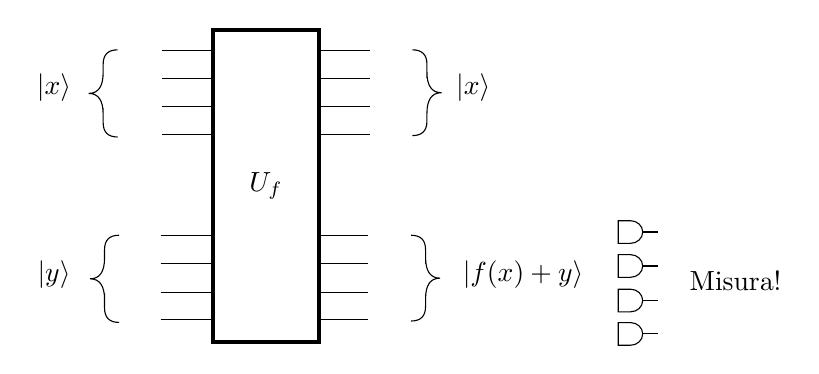
\begin{tikzpicture}[x=0.75pt,y=0.75pt,yscale=-1,xscale=1]
%uncomment if require: \path (0,300); %set diagram left start at 0, and has height of 300

%Straight Lines [id:da22244990805952436] 
\draw    (177.67,131.33) -- (202.46,131.33) ;


%Straight Lines [id:da0959742164698143] 
\draw    (177.67,118.11) -- (202.46,118.11) ;


%Straight Lines [id:da35646456098851287] 
\draw    (177.67,104.44) -- (202.46,104.44) ;


%Straight Lines [id:da9495010153773733] 
\draw    (177.67,91) -- (202.46,91) ;


%Shape: Rectangle [id:dp037145220774647214] 
\draw  [line width=1.5]  (202.46,81) -- (253.2,81) -- (253.2,231.33) -- (202.46,231.33) -- cycle ;
%Straight Lines [id:da7090506996054302] 
\draw    (177,220.67) -- (201.79,220.67) ;


%Straight Lines [id:da8160422595152328] 
\draw    (177,207.45) -- (201.79,207.45) ;


%Straight Lines [id:da8238964572049521] 
\draw    (177,193.78) -- (201.79,193.78) ;


%Straight Lines [id:da581995668864403] 
\draw    (177,180.33) -- (201.79,180.33) ;


%Straight Lines [id:da23327546799574295] 
\draw    (253.65,131.33) -- (277.67,131.33) ;


%Straight Lines [id:da6156361724592183] 
\draw    (253.65,118.11) -- (277.67,118.11) ;


%Straight Lines [id:da9907572422653355] 
\draw    (253.65,104.44) -- (277.67,104.44) ;


%Straight Lines [id:da2000446500452704] 
\draw    (253.65,91) -- (277.67,91) ;


%Straight Lines [id:da8225100479741072] 
\draw    (253,220.67) -- (277.02,220.67) ;


%Straight Lines [id:da8242637192553153] 
\draw    (253,207.45) -- (277.02,207.45) ;


%Straight Lines [id:da9855008133144141] 
\draw    (253,193.78) -- (277.02,193.78) ;


%Straight Lines [id:da20317136628817978] 
\draw    (253,180.33) -- (277.02,180.33) ;


%Shape: Brace [id:dp42724719204409056] 
\draw   (156.33,90.67) .. controls (151.66,90.67) and (149.33,93) .. (149.33,97.67) -- (149.33,101.67) .. controls (149.33,108.34) and (147,111.67) .. (142.33,111.67) .. controls (147,111.67) and (149.33,115) .. (149.33,121.67)(149.33,118.67) -- (149.33,125.67) .. controls (149.33,130.34) and (151.66,132.67) .. (156.33,132.67) ;
%Shape: Brace [id:dp4995708102634657] 
\draw   (157,180) .. controls (152.33,180) and (150,182.33) .. (150,187) -- (150,191) .. controls (150,197.67) and (147.67,201) .. (143,201) .. controls (147.67,201) and (150,204.33) .. (150,211)(150,208) -- (150,215) .. controls (150,219.67) and (152.33,222) .. (157,222) ;
%Shape: Brace [id:dp6295223754766166] 
\draw   (298.33,132) .. controls (303,132) and (305.33,129.67) .. (305.33,125) -- (305.33,121.33) .. controls (305.33,114.66) and (307.66,111.33) .. (312.33,111.33) .. controls (307.66,111.33) and (305.33,108) .. (305.33,101.33)(305.33,104.33) -- (305.33,97.67) .. controls (305.33,93) and (303,90.67) .. (298.33,90.67) ;
%Shape: Brace [id:dp3197890304445641] 
\draw   (297.67,221.33) .. controls (302.34,221.33) and (304.67,219) .. (304.67,214.33) -- (304.67,210.67) .. controls (304.67,204) and (307,200.67) .. (311.67,200.67) .. controls (307,200.67) and (304.67,197.34) .. (304.67,190.67)(304.67,193.67) -- (304.67,187) .. controls (304.67,182.33) and (302.34,180) .. (297.67,180) ;
%Flowchart: Delay [id:dp7276420652755575] 
\draw   (397.5,222.09) -- (403.39,222.09) .. controls (406.65,222.09) and (409.28,224.53) .. (409.28,227.55) .. controls (409.28,230.56) and (406.65,233) .. (403.39,233) -- (397.5,233) -- cycle ;
%Flowchart: Delay [id:dp7667317499565782] 
\draw   (397.5,206) -- (403.39,206) .. controls (406.65,206) and (409.28,208.44) .. (409.28,211.45) .. controls (409.28,214.47) and (406.65,216.91) .. (403.39,216.91) -- (397.5,216.91) -- cycle ;
%Flowchart: Delay [id:dp04570126715135392] 
\draw   (397.5,189.36) -- (403.39,189.36) .. controls (406.65,189.36) and (409.28,191.81) .. (409.28,194.82) .. controls (409.28,197.83) and (406.65,200.27) .. (403.39,200.27) -- (397.5,200.27) -- cycle ;
%Flowchart: Delay [id:dp4268839193937979] 
\draw   (397.5,173) -- (403.39,173) .. controls (406.65,173) and (409.28,175.44) .. (409.28,178.45) .. controls (409.28,181.47) and (406.65,183.91) .. (403.39,183.91) -- (397.5,183.91) -- cycle ;
%Straight Lines [id:da0645520339063792] 
\draw    (409.28,178.45) -- (416.5,178.45) ;


%Straight Lines [id:da31065648181109173] 
\draw    (409.28,194.82) -- (416.5,194.82) ;


%Straight Lines [id:da6262618451334159] 
\draw    (409.28,211.45) -- (416.5,211.45) ;


%Straight Lines [id:da31986129480109327] 
\draw    (409.28,227.55) -- (416.5,227.55) ;



% Text Node
\draw (227.83,156.17) node   {$U_{f}$};
% Text Node
\draw (125.67,109) node   {$|x\rangle $};
% Text Node
\draw (125.67,199) node   {$|y\rangle $};
% Text Node
\draw (327.67,109) node   {$|x\rangle $};
% Text Node
\draw (351.67,199) node   {$|f( x) +y\rangle $};
% Text Node
\draw (454,202) node  [align=left] {Misura!};


\end{tikzpicture}
\end{center}
\caption{Seppure una computazione quantistica possa avvenire in \q{parallelo} su tutte le singole configurazioni di cui lo stato iniziale è combinazione lineare, per poter \q{usare} l'output è necessario effettuare una misura, che collassa lo stato finale $\ket{\psi_o} = \sum_{x=0}^{2^n-1}c_x \ket{x}\ket{y+f(x)}$ in \textbf{uno solo} dei $2^n$ esiti possibili, con probabilità $|c_x|^2$\label{fig:quantum-parallelism}}
\end{figure}

Si prospetta però la possibilità di regolare opportunamente lo stato finale in modo che l'esito desiderato sia quello dominante, ossia con la maggiore probabilità di presentarsi. In tal modo si può ottenere (con alta probabilità) la risposta voluta.

\subsection{Esempio di funzione quantistica}
Assumiamo\index{Esempio!Circuito per stato di massima sovrapposizione} di poter configurare $n$ qubit nello stato $\ket{0000\dots0}$. Vogliamo trovare un'operazione per farlo evolvere a uno stato del tipo:
\begin{align*}
\underbrace{\ket{0000\dots0}}_{n} \mapsto \frac{1}{\sqrt{2^n}} \sum_{x=0}^{2^n-1} \ket{x}
\end{align*}

Per esempio, nel caso $n=2$ avremo:
\begin{align*}
\ket{00} \mapsto \frac{1}{2}(\ket{00}+\ket{01}+\ket{10}+\ket{11})
\end{align*}
Stiamo cioè mappando uno stato \textit{nullo} in una combinazione lineare di \textit{tutti gli stati possibili} a pari coefficienti. Un modo per far ciò consiste nell'usare $n$ porte Hadamard:



\tikzset{every picture/.style={line width=0.75pt}} %set default line width to 0.75pt        
\begin{center}
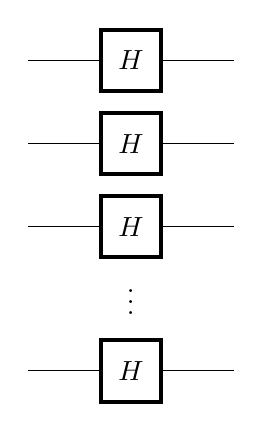
\begin{tikzpicture}[x=0.75pt,y=0.75pt,yscale=-1,xscale=1]
%uncomment if require: \path (0,300); %set diagram left start at 0, and has height of 300

%Straight Lines [id:da10448720978738102] 
\draw    (216.17,95.83) -- (315.17,95.83) ;


%Shape: Rectangle [id:dp11213822137435825] 
\draw  [fill={rgb, 255:red, 255; green, 255; blue, 255 }  ,fill opacity=1 ][line width=1.5]  (251.13,81) -- (280.21,81) -- (280.21,110.67) -- (251.13,110.67) -- cycle ;
%Straight Lines [id:da9310952190394066] 
\draw    (216.17,135.83) -- (315.17,135.83) ;


%Shape: Rectangle [id:dp05924388127440561] 
\draw  [fill={rgb, 255:red, 255; green, 255; blue, 255 }  ,fill opacity=1 ][line width=1.5]  (251.13,121) -- (280.21,121) -- (280.21,150.67) -- (251.13,150.67) -- cycle ;
%Straight Lines [id:da8309244851731774] 
\draw    (216.17,175.83) -- (315.17,175.83) ;


%Shape: Rectangle [id:dp37953417452095795] 
\draw  [fill={rgb, 255:red, 255; green, 255; blue, 255 }  ,fill opacity=1 ][line width=1.5]  (251.13,161) -- (280.21,161) -- (280.21,190.67) -- (251.13,190.67) -- cycle ;
%Straight Lines [id:da714375072170162] 
\draw    (216.17,245.33) -- (315.17,245.33) ;


%Shape: Rectangle [id:dp29674138337370226] 
\draw  [fill={rgb, 255:red, 255; green, 255; blue, 255 }  ,fill opacity=1 ][line width=1.5]  (251.13,230.5) -- (280.21,230.5) -- (280.21,260.17) -- (251.13,260.17) -- cycle ;

% Text Node
\draw (265.67,95.83) node   {$H$};
% Text Node
\draw (265.67,135.83) node   {$H$};
% Text Node
\draw (265.67,175.83) node   {$H$};
% Text Node
\draw (265.67,245.33) node   {$H$};
% Text Node
\draw (265.5,208) node   {$\vdots $};


\end{tikzpicture}
\end{center}

Riscriviamo l'azione di $H$ in modo compatto come:\index{Porte logiche!Hadamard}
\begin{align*}
H\ket{x} = \frac{1}{\sqrt{2}} \sum_{y=0,1} (-1)^{xy} \ket{y}
\end{align*}
che riproduce la stessa casistica definita in precedenza. Infatti se $x = 0$, allora $(-1)^0=1$ per un qualsiasi valore di $y$, e quindi avremo $H\ket{0} = (\ket{0}+\ket{1})/\sqrt{2}$, mentre per $x=1$ avremo un $(-1)$ quando anche $y=1$, e quindi $H\ket{1}=(\ket{0}-\ket{1})/\sqrt{2}$, come richiesto.\\

Se abbiamo due qubit, $\ket{x_1}$ e $\ket{x_2}$, e li mandiamo ciascuno attraverso una $H$, otteniamo:
\begin{align*}
(H\otimes H)\ket{x_1} \ket{x_2} &= \frac{1}{\sqrt{2}}\left(\sum_{y_1} (-1)^{x_1 y_1} \ket{y_1}\right)\frac{1}{\sqrt{2}}\left(\sum_{y_2}(-1)^{x_2y_2}\ket{y_2}\right)=\\
&=\frac{1}{2} \left(\sum_{y_1 y_2} (-1)^{x_1 y_1 + x_2y_2} \ket{y_1}\ket{y_2}\right)
\end{align*}
Generalizzando a $n$ qubit, e schematizzando la somma dei prodotti di bit corrispondenti con un \textit{prodotto scalare} $\vec{x}\cdot \vec{y}$, con $\vec{x}$ e $\vec{y}$ vettori di bit:
\begin{align*}
(H\otimes \dots \otimes H) \ket{x_1}\dots \ket{x_n} = \frac{1}{(\sqrt{2})^n} \sum (-1)^{\vec{x}\cdot \vec{y}}\ket{y_1, \dots, y_n} = \frac{1}{\sqrt{2^n}} \sum_{y=0}^{2^n-1} (-1)^{\vec{x}\cdot\vec{y}} \ket{\vec{y}}
\end{align*}

Nel caso che $\vec{x}=(0,\dots,0)$  il coefficiente $(-1)^{\vec{x}\cdot \vec{y}}$ sparisce, e quindi otteniamo l'output desiderato:
\begin{align*}
\ket{\psi_{f}}=\sum_{y=0}^{2^n-1} \ket{\vec{y}}
\end{align*}

\textbf{Nota}: nonostante la complessità della forma finale, non si ha alcuna correlazione tra i vari qubit - infatti lo stato finale è un prodotto tensore di $H$ applicate ciascuna a \textit{una singola entrata}, ossia \textbf{non è} uno stato entangled. Pittorescamente: stiamo agendo sui singoli qubit \textit{uno alla volta}, e quindi nessuno \q{è a conoscenza} dello stato degli altri - perciò non possono esservi effetti di interferenza.

\section{No cloning theorem}
Abbiamo accennato che in \MQ non è possibile copiare esattamente uno stato. Esaminiamo ora tale questione\index{Teorema!No cloning}.\\

Possiamo trovare un'operazione che possa copiare uno stato $\ket{\psi}$, indipendentemente dallo stato? Formalmente, vogliamo scrivere una certa $U$ tale che:
\begin{align}
U\ket{\psi}\ket{0} = \ket{\psi}\ket{\psi} \qquad U \text{ unitaria}, \forall \ket{\psi} \label{eqn:Ucopy}
\end{align}
(dove stiamo usando due registri di pari dimensione per garantire l'unitarietà dell'operazione).

\begin{figure}[H]
\centering


\tikzset{every picture/.style={line width=0.75pt}} %set default line width to 0.75pt        
\begin{center}
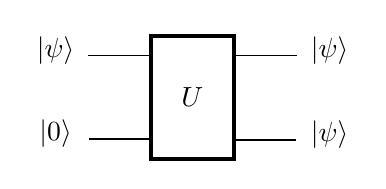
\begin{tikzpicture}[x=0.75pt,y=0.75pt,yscale=-1,xscale=1]
%uncomment if require: \path (0,300); %set diagram left start at 0, and has height of 300

%Shape: Rectangle [id:dp5049814893934905] 
\draw  [line width=1.5]  (220,120.5) -- (259.75,120.5) -- (259.75,179.5) -- (220,179.5) -- cycle ;
%Straight Lines [id:da7877497388492118] 
\draw    (189.75,130) -- (219.75,130) ;


%Straight Lines [id:da009334325250696995] 
\draw    (190.25,170) -- (220.25,170) ;


%Straight Lines [id:da9491833456963361] 
\draw    (260.25,130) -- (290.25,130) ;


%Straight Lines [id:da9179785583004338] 
\draw    (259.75,170.5) -- (289.75,170.5) ;



% Text Node
\draw (174,127.5) node   {$|\psi \rangle $};
% Text Node
\draw (174,167.5) node   {$|0\rangle $};
% Text Node
\draw (306,127.5) node   {$|\psi \rangle $};
% Text Node
\draw (306,168) node   {$|\psi \rangle $};
% Text Node
\draw (239.88,150) node   {$U$};


\end{tikzpicture}
\end{center}
\caption{Schema di una porta logica \textit{copy} quantistica\label{fig:copy-mq}}
\end{figure}

Il \textbf{no cloning theorem} afferma che tale $U$ \textbf{non esiste}.\\

Dimostriamolo.\marginpar{Dimostrazione} Supponiamo che esista una $U$ del genere, per cui $\forall \ket{\psi}$ vale $U\ket{\psi}\ket{0} = \ket{\psi}\ket{\psi}$. Consideriamo due stati $\ket{\Psi_1}=\ket{\psi}\ket{0}$ e $\ket{\Psi_2}=\ket{\varphi}\ket{0}$. Applicando $U$ a ciascuno di essi si ha:
\begin{align}
\ket{\Phi_1} &= U\ket{\Psi_1}=
U\ket{\psi}\ket{0} \underset{(\ref{eqn:Ucopy})}{=} \ket{\psi}\ket{\psi} \nonumber\\
\ket{\Phi_2} &= U\ket{\Psi_2} =
U\ket{\varphi}\ket{0}  \underset{(\ref{eqn:Ucopy})}{=} \ket{\varphi}\ket{\varphi}
\label{eqn:Udef}
\end{align}
Calcoliamo il prodotto scalare dei due stati finali:
\begin{align*}
P = \braket{\Phi_2|\Phi_1}
\end{align*}
Abbiamo due modi per farlo:
\begin{itemize}
\item Usiamo per $\ket{\Phi_1}$ e $\ket{\Phi_2}$ l'espressione in termini di $U$ unitario.
\begin{align*}
P = \bra{\varphi}\bra{0}U^\dag U \ket{\psi}\ket{0} \underset{(a)}{=} \bra{\varphi}\braket{0|\psi}\ket{0} = \braket{\varphi|\psi}
\end{align*}
dove in (a) si è usata l'unitarietà di $U$, per cui vale $U^\dag U = \bb{I}$.

\item Usiamo la definizione di $U$, ossia la (\ref{eqn:Udef}):
\begin{align*}
P = \bra{\varphi}\braket{\varphi|\psi}\ket{\psi} = \braket{\varphi|\psi}^2
\end{align*}
\end{itemize}
Ma allora deve essere:
\begin{align*}
\braket{\varphi|\psi} = \braket{\varphi|\psi}^2
\end{align*}
cosa che \textbf{non è vera} in generale per ogni stato. Perciò \textit{non è possibile} clonare un generico stato senza conoscerlo.\\
Dal risultato trovato, tuttavia, notiamo che stati ortogonali, per cui $\braket{\varphi|\psi}=0$, possono però essere clonati senza problemi: possiamo quindi clonare tutti gli stati \textit{di una base ortonormale}, ma non le loro generiche combinazioni (che formano stati generici).

\section{Classi di complessità algoritmica}
I computer quantistici permettono di raggiungere una maggiore efficienza rispetto ai computer classici. Per quantificare tale fenomeno si utilizza una definizione di \textbf{classi di complessità}\index{Classi di complessità}, che permettono di quantificare \q{quanto un algoritmo è complesso}. L'idea è quella di esaminare come la quantità di tempo/risorse necessarie a risolvere un problema \textit{scali} al crescere della dimensione del problema.\\
Per esempio, se consideriamo un algoritmo per scomporre un numero in numeri primi, la sua complessità è legata a \textit{quanto velocemente} il tempo o le risorse necessarie alla computazione crescano all'aumentare del \textit{numero di cifre} del numero dato in input.\\
Si trova che, in generale, \textit{tempo} e \textit{risorse} (la \q{memoria} utilizzata dal computer) sono correlate tra loro: è possibile usare più di una per compensare l'altra. Tuttavia, un problema di una certa complessità richiede in ogni caso una certa quantità minima \textit{globale} di risorse.\\

In particolare, consideriamo la funzione $f(n)$ che, data la grandezza $n$ dell'input, ossia il \textit{numero di bit} in ingresso, computa la \textbf{quantità di risorse necessarie} alla computazione. Abbiamo due possibilità:\marginpar{Problemi facili e difficili}
\begin{itemize}
\item $f(n)$ ha un andamento \textbf{polinomiale} in $n$ (P), cioè è maggiorabile con un polinomio: $\exists N\in \bb{N}$ t.c. $f(n) \leq n^N$ definitivamente.\\
I problemi in cui le risorse scalano in modo polinomiale sono considerati \textbf{facili}.
\item Se invece la funzione è \textbf{superpolinomiale}, cioè cresce più velocemente di ogni polinomio, il problema è ritenuto \textbf{difficile}.
\end{itemize}

Troviamo quindi tre classi:\marginpar{Classi P, NP, NPC}
\begin{itemize}
\item \textbf{P}: problemi risolvibili in tempo \textbf{polinomiale}.
\item \textbf{NP}: \textit{Non-deterministic Polynomial time}. Si tratta di problemi che una macchina di Turing non deterministica (che specifichiamo più avanti) può risolvere in tempo polinomiale. Si trova che i problemi NP corrispondono anche ai problemi la cui soluzione può essere \textbf{verificata} in tempo polinomiale da una macchina di Turing deterministica (cioè si ha che fare con \q{soluzioni ovvie a posteriori ma difficili da trovare in primo luogo}).
\item \textbf{NPC}: \textit{NP-Complete}, è composta da problemi la cui soluzione può essere riadattata \textit{in tempo polinomiale} alla soluzione di un problema NP. In altre parole, gli NPC sono almeno tanto difficili quanto il più difficile degli NP, e trovando un algoritmo polinomiale che risolva un solo NPC è automaticamente possibile risolvere tutti gli NP sempre in tempo polinomiale, semplicemente riadattando opportunamente la soluzione trovata.
\end{itemize}

La \textbf{macchina di Turing}\marginpar{Macchina di Turing}\index{Macchina di turing} è l'oggetto astratto che \textit{schematizza} l'azione di ogni computer. Consideriamo un \textit{nastro infinito}, diviso in \textit{cellette} che fungono da \textbf{registri}, su cui una macchina può scrivere con un certo \textit{alfabeto} fissato (che può essere per esempio quello binario).

\begin{figure}[H]
\centering


\tikzset{every picture/.style={line width=0.75pt}} %set default line width to 0.75pt        
\begin{center}
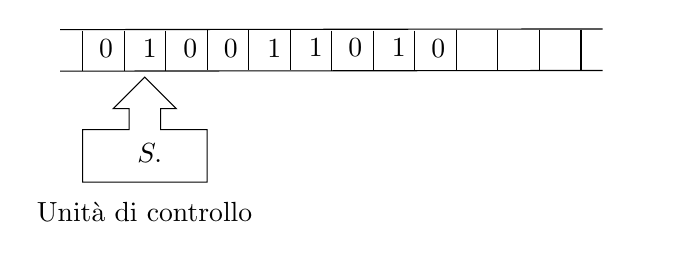
\begin{tikzpicture}[x=0.75pt,y=0.75pt,yscale=-1,xscale=1]
%uncomment if require: \path (0,300); %set diagram left start at 0, and has height of 300

%Straight Lines [id:da7275362281558355] 
\draw    (189.33,120) -- (450.67,119.67) ;


%Straight Lines [id:da29120625547318935] 
\draw    (189.33,140) -- (450.67,139.67) ;


%Straight Lines [id:da7625664285601652] 
\draw    (200.25,120.5) -- (200.25,140) ;


%Straight Lines [id:da10240131930295271] 
\draw    (220.25,120.5) -- (220.25,140) ;


%Straight Lines [id:da978604948835289] 
\draw    (240.25,120.5) -- (240.25,140) ;


%Straight Lines [id:da9959379734940303] 
\draw    (260.25,120) -- (260.25,139.5) ;


%Straight Lines [id:da9581700306481775] 
\draw    (280.25,120) -- (280.25,139.5) ;


%Straight Lines [id:da4437031266260554] 
\draw    (300.25,120) -- (300.25,139.5) ;


%Straight Lines [id:da6017637495165318] 
\draw    (320.25,120.5) -- (320.25,140) ;


%Straight Lines [id:da5089858317275813] 
\draw    (340.25,120.5) -- (340.25,140) ;


%Straight Lines [id:da043107959414806274] 
\draw    (360.25,120.5) -- (360.25,140) ;


%Straight Lines [id:da724113904491829] 
\draw    (380.25,120) -- (380.25,139.5) ;


%Straight Lines [id:da049275772796910644] 
\draw    (400.25,120) -- (400.25,139.5) ;


%Straight Lines [id:da6822986153958353] 
\draw    (420.25,120) -- (420.25,139.5) ;


%Straight Lines [id:da0016020051178489148] 
\draw    (440.25,120) -- (440.25,139.5) ;


%Callout Right Arrow [id:dp576862285756073] 
\draw   (200.13,193.5) -- (200.13,168.19) -- (222.53,168.19) -- (222.53,158.06) -- (214.94,158.06) -- (230.13,142.88) -- (245.31,158.06) -- (237.72,158.06) -- (237.72,168.19) -- (260.13,168.19) -- (260.13,193.5) -- cycle ;

% Text Node
\draw (211.5,129) node   {$0$};
% Text Node
\draw (232.5,129) node   {$1$};
% Text Node
\draw (252,129) node   {$0$};
% Text Node
\draw (271.5,129) node   {$0$};
% Text Node
\draw (292.5,129) node   {$1$};
% Text Node
\draw (312.5,128.5) node   {$1$};
% Text Node
\draw (331.5,128.5) node   {$0$};
% Text Node
\draw (473,123.5) node   {$\dotsc $};
% Text Node
\draw (232.5,179.5) node   {$S.$};
% Text Node
\draw (230,208) node  [align=left] {Unità di controllo};
% Text Node
\draw (352.5,128.5) node   {$1$};
% Text Node
\draw (371.5,129) node   {$0$};


\end{tikzpicture}
\end{center}
\caption{Schema della macchina di Turing\label{fig:turing}}
\end{figure}

Sul nastro agisce, tramite operazioni di \textbf{lettura/scrittura}, una \textbf{unità di controllo} $S$, che consiste in una \textbf{macchina a stati finiti}. Ciò significa che $S$ può trovarsi, in un dato istante, in uno di $N<\infty$ stati possibili. Ogni stato definisce il comportamento della macchina, e vi sono \textit{regole} per passare da uno stato all'altro. Un esempio di comportamento associato ad uno stato potrebbe essere \q{leggi il bit corrente}, oppure \q{fai scorrere di $1$ il nastro in avanti}. Tra questi stati possibili vi è lo stato \textbf{halt} (H), che indica il \textbf{termine dell'esecuzione} del programma.\\

In particolare, una macchina di Turing\marginpar{Macchine di Turing (non) deterministiche} \textbf{deterministica} è tale che le regole di passaggio da uno stato all'altro dell'unità di controllo sono deterministiche, ossia conoscendo lo stato corrente $A$ e il valore di registro a cui la macchina ha accesso si sa automaticamente il valore del prossimo stato $B$ che assumerà $S$. Se invece è possibile solo dare una \textit{probabilità} per i passaggi di stato, la macchina è \textbf{non deterministica}. Avendo una maggiore libertà d'azione, una macchina non deterministica è \textit{più potente} di una deterministica.\\

Notiamo infine che non sappiamo la \textbf{gerarchia} delle classi di complessità, ossia non è chiaro se \textbf{NP} e \textbf{P} siano in realtà lo stesso insieme, cioè se esista o meno un algoritmo \textit{efficiente} per risolvere \textit{problemi difficili}. \marginpar{P=NP?}

\begin{figure}[H]
\centering


\tikzset{every picture/.style={line width=0.75pt}} %set default line width to 0.75pt        
\begin{center}
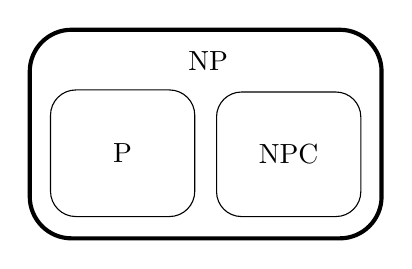
\begin{tikzpicture}[x=0.75pt,y=0.75pt,yscale=-1,xscale=1]
%uncomment if require: \path (0,300); %set diagram left start at 0, and has height of 300

%Rounded Rect [id:dp4469509270957106] 
\draw  [line width=1.5]  (180.5,110.1) .. controls (180.5,99) and (189.5,90) .. (200.6,90) -- (329.9,90) .. controls (341,90) and (350,99) .. (350,110.1) -- (350,170.4) .. controls (350,181.5) and (341,190.5) .. (329.9,190.5) -- (200.6,190.5) .. controls (189.5,190.5) and (180.5,181.5) .. (180.5,170.4) -- cycle ;
%Rounded Rect [id:dp019097988645257136] 
\draw   (190.5,131.2) .. controls (190.5,124.46) and (195.96,119) .. (202.7,119) -- (247.8,119) .. controls (254.54,119) and (260,124.46) .. (260,131.2) -- (260,167.8) .. controls (260,174.54) and (254.54,180) .. (247.8,180) -- (202.7,180) .. controls (195.96,180) and (190.5,174.54) .. (190.5,167.8) -- cycle ;
%Rounded Rect [id:dp3526831805757056] 
\draw   (270.5,132) .. controls (270.5,125.37) and (275.87,120) .. (282.5,120) -- (328,120) .. controls (334.63,120) and (340,125.37) .. (340,132) -- (340,168) .. controls (340,174.63) and (334.63,180) .. (328,180) -- (282.5,180) .. controls (275.87,180) and (270.5,174.63) .. (270.5,168) -- cycle ;

% Text Node
\draw (266.5,105) node  [align=left] {NP};
% Text Node
\draw (225.25,149.5) node  [align=left] {P};
% Text Node
\draw (305.25,150) node  [align=left] {NPC};


\end{tikzpicture}
\end{center}
\caption{Attualmente sappiamo che NP$\subset$NPC, e P$\subset$NP, ma non è chiaro se valgano (eventualmente) inclusioni inverse.\label{fig:n-np-npc}}
\end{figure}

Considerando macchine di Turing non deterministiche, consideriamo altre classi di complessità:
\begin{itemize}
\item \textbf{BPP}: \textit{Bounded Error Probabilistic Polynomial}. Un problema è in BPP se esiste un algoritmo polinomiale che dà il risultato giusto con una probabilità migliore del caso, ossia con $p=\frac{1}{2}+\delta$, con $\delta >0$. Basta infatti tale \textit{bias} per poter ripetere (in tempo polinomiale) l'algoritmo, migliorando \q{quanto si vuole} la probabilità di successo.
\item \textbf{BQP}: \textit{Bounded error Quantum Probabilistic Polynomial}. Un problema è in BQP se è risolvibile da un \textit{computer quantistico} con una probabilità leggermente biased ($p=\frac{1}{2}+\delta$, $\delta >0$). Per esempio, l'algoritmo di Shor per la fattorizzazione di numeri primi è di questo tipo.
\end{itemize}

Anche qui non sappiamo se tali insiemi siano gli stessi. Di sicuro vale:
\begin{align*}
\op{P} \subseteq \op{BPP} \subseteq \op{BQP}
\end{align*}
Vi sono attualmente algoritmi quantistici \textit{più performanti} di ogni algoritmo classico, ma nulla impedisce che in futuro si trovino nuovi algoritmi classici ancora più efficienti. Non è quindi ancora certo che i computer quantistici siano \textit{a priori} in grado di superare i computer classici.

\section{Esercizio \theEsercizio}\stepcounter{Esercizio}
\index{Esercizio!Circuito per stato generico}
Vogliamo verificare che uno stato generico di un qubit possa essere realizzato partendo da $\ket{0}$ e applicando una precisa sequenza di gate:
\begin{align*}
\ket{\psi} &= \cos\frac{\theta}{2} \ket{0} + e^{i\varphi} \sin\frac{\theta}{2}\ket{1}=\\
&= R_z\left(\frac{\pi}{2}+\varphi\right)HR_z(\theta) H \ket{0}
\end{align*}
\marginpar{[Controllare il segno di $\varphi$]}

Graficamente ciò corrisponde a realizzare il circuito:



\tikzset{every picture/.style={line width=0.75pt}} %set default line width to 0.75pt        
\begin{center}
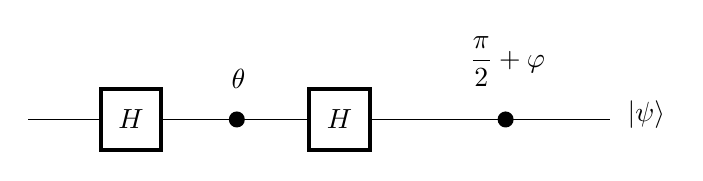
\begin{tikzpicture}[x=0.75pt,y=0.75pt,yscale=-1,xscale=1]
%uncomment if require: \path (0,300); %set diagram left start at 0, and has height of 300

%Straight Lines [id:da06979007227355538] 
\draw    (140.17,140.33) -- (239.17,140.33) ;


%Shape: Rectangle [id:dp49376768989171205] 
\draw  [fill={rgb, 255:red, 255; green, 255; blue, 255 }  ,fill opacity=1 ][line width=1.5]  (175.13,125.5) -- (204.21,125.5) -- (204.21,155.17) -- (175.13,155.17) -- cycle ;
%Straight Lines [id:da007553374828097148] 
\draw    (240.67,140.33) -- (370.17,140.33) ;

\draw [shift={(240.67,140.33)}, rotate = 360] [color={rgb, 255:red, 0; green, 0; blue, 0 }  ][fill={rgb, 255:red, 0; green, 0; blue, 0 }  ][line width=0.75]      (0, 0) circle [x radius= 3.35, y radius= 3.35]   ;
%Shape: Rectangle [id:dp522626456344331] 
\draw  [fill={rgb, 255:red, 255; green, 255; blue, 255 }  ,fill opacity=1 ][line width=1.5]  (275.63,125.5) -- (304.71,125.5) -- (304.71,155.17) -- (275.63,155.17) -- cycle ;
%Straight Lines [id:da11299120546483388] 
\draw    (370.17,140.33) -- (420.42,140.33) ;

\draw [shift={(370.17,140.33)}, rotate = 0] [color={rgb, 255:red, 0; green, 0; blue, 0 }  ][fill={rgb, 255:red, 0; green, 0; blue, 0 }  ][line width=0.75]      (0, 0) circle [x radius= 3.35, y radius= 3.35]   ;

% Text Node
\draw (189.67,140.33) node   {$H$};
% Text Node
\draw (290.17,140.33) node   {$H$};
% Text Node
\draw (438,138) node   {$|\psi \rangle $};
% Text Node
\draw (241.5,121) node   {$\theta $};
% Text Node
\draw (371,112.5) node  [align=left] {$\displaystyle \frac{\pi }{2} +\varphi $};


\end{tikzpicture}
\end{center}

Svolgiamo il conto, per esempio usando le rappresentazioni matriciali:
\begin{align*}
H = \frac{1}{\sqrt{2}}\begin{pmatrix}
1 & 1\\
1 & -1
\end{pmatrix} \qquad R_z(\delta)= \begin{pmatrix} 1 & 0\\ 0 & e^{i\delta} \end{pmatrix}
\end{align*}
Nella base computazionale ricordiamo che:
\begin{align*}
\ket{0} = \begin{pmatrix}1 \\ 0 \end{pmatrix} \qquad \ket{1} = \begin{pmatrix}0 \\ 1 \end{pmatrix}
\end{align*}
Applichiamo allora le porte logiche una dopo l'altra, svolgendo di volta in volta le moltiplicazioni \textit{matrice per vettore}:
\begin{align*}
\ket{0} = \begin{pmatrix} 1 \\ 0 \end{pmatrix} \xrightarrow{H}{} \frac{1}{\sqrt{2}}\begin{pmatrix}1\\1\end{pmatrix}\xrightarrow{R_z(\theta)}{} \frac{1}{\sqrt{2}}\begin{pmatrix}1 \\ e^{i\theta}\end{pmatrix} \xrightarrow{H}{} \begin{pmatrix}\frac{1+e^{i\theta}}{2}\\ \frac{1-e^{i\theta}}{2}\end{pmatrix}=
e^{i\frac{\theta}{2}} \begin{pmatrix}
\frac{e^{i\theta/2}+e^{-i\theta/2}}{2}\\
\frac{-e^{i\theta/2}+e^{-i\theta/2}}{2\textcolor{Red}{i}}\textcolor{Red}{i}
\end{pmatrix}=\\
\underset{(a)}{=}
\bcancel{e^{i\frac{\theta}{2}}}\begin{pmatrix}
\cos\frac{\theta}{2}\\\smash[t]{\underbrace{-i}_{e^{-i\pi/2}}}\sin\frac{\theta}{2}
\end{pmatrix} \xrightarrow{R_z\left(\frac{\pi}{2}+\varphi\right)} \left[ \cos\frac{\theta}{2}\ket{0} + \exp\left(i\frac{\pi}{2} +i\varphi -i\frac{\pi}{2}\right)\sin\frac{\theta}{2} \ket{1}\right] =\\
= \cos\frac{\theta}{2}\ket{0} + e^{i\varphi}\sin\frac{\theta}{2}\ket{1}\span
\end{align*}
In (a) rimuoviamo la fase globale (che non cambia lo stato).

\section{Esercizio \theEsercizio}\stepcounter{Esercizio}
\index{Esercizio!CPHASE in termini di CNOT e phase-shift}
Vogliamo verificare che l'operatore $\delta$ (C-PHASE) definito dalla matrice:
\begin{align*}
\delta = \left(
        \begin{array}{cc|cc}
        1 & 0 & 0 & 0 \\
        0 & 1 & 0 & 0 \\
        \hline
        0 & 0 & 1 & 0 \\
        0 & 0 & 0 & e^{i\delta} \\        
        \end{array}
\right) 
\end{align*}
può essere ottenuto dalla combinazione di $5$ porte logiche fondamentali (CNOT e phase-shift) come schematizzato in figura:
\begin{figure}[H]
\centering


\tikzset{every picture/.style={line width=0.75pt}} %set default line width to 0.75pt        
\begin{center}
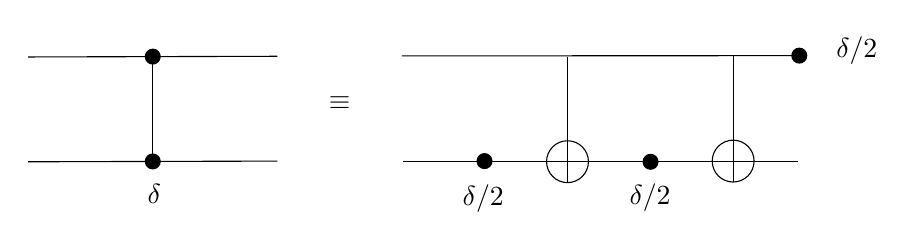
\begin{tikzpicture}[x=0.75pt,y=0.75pt,yscale=-1,xscale=1]
%uncomment if require: \path (0,300); %set diagram left start at 0, and has height of 300

%Straight Lines [id:da21074801917912667] 
\draw    (130.5,140.5) -- (250.5,140.17) ;


%Straight Lines [id:da9874287036079263] 
\draw    (190.5,140.33) -- (190.5,190.83) ;
\draw [shift={(190.5,190.83)}, rotate = 90] [color={rgb, 255:red, 0; green, 0; blue, 0 }  ][fill={rgb, 255:red, 0; green, 0; blue, 0 }  ][line width=0.75]      (0, 0) circle [x radius= 3.35, y radius= 3.35]   ;
\draw [shift={(190.5,140.33)}, rotate = 90] [color={rgb, 255:red, 0; green, 0; blue, 0 }  ][fill={rgb, 255:red, 0; green, 0; blue, 0 }  ][line width=0.75]      (0, 0) circle [x radius= 3.35, y radius= 3.35]   ;
%Straight Lines [id:da4830080618133892] 
\draw    (130.5,191) -- (250.5,190.67) ;


%Straight Lines [id:da1548073386756772] 
\draw    (310.5,140) -- (502,139.86) ;
\draw [shift={(502,139.86)}, rotate = 359.96] [color={rgb, 255:red, 0; green, 0; blue, 0 }  ][fill={rgb, 255:red, 0; green, 0; blue, 0 }  ][line width=0.75]      (0, 0) circle [x radius= 3.35, y radius= 3.35]   ;

%Straight Lines [id:da4883105543582402] 
\draw    (390.32,140.45) -- (390.32,190.95) ;


%Straight Lines [id:da26794551989187454] 
\draw    (311.17,190.67) -- (501.17,190.67) ;


%Straight Lines [id:da5454348469497672] 
\draw    (470.13,140.17) -- (470.13,190.67) ;


%Flowchart: Or [id:dp42872792207775023] 
\draw  [fill={rgb, 255:red, 255; green, 255; blue, 255 }  ,fill opacity=1 ] (380.23,190.95) .. controls (380.23,185.38) and (384.75,180.87) .. (390.32,180.87) .. controls (395.88,180.87) and (400.4,185.38) .. (400.4,190.95) .. controls (400.4,196.52) and (395.88,201.04) .. (390.32,201.04) .. controls (384.75,201.04) and (380.23,196.52) .. (380.23,190.95) -- cycle ; \draw   (380.23,190.95) -- (400.4,190.95) ; \draw   (390.32,180.87) -- (390.32,201.04) ;
%Flowchart: Or [id:dp5893976293181182] 
\draw  [fill={rgb, 255:red, 255; green, 255; blue, 255 }  ,fill opacity=1 ] (460.04,190.67) .. controls (460.04,185.1) and (464.56,180.58) .. (470.13,180.58) .. controls (475.69,180.58) and (480.21,185.1) .. (480.21,190.67) .. controls (480.21,196.24) and (475.69,200.75) .. (470.13,200.75) .. controls (464.56,200.75) and (460.04,196.24) .. (460.04,190.67) -- cycle ; \draw   (460.04,190.67) -- (480.21,190.67) ; \draw   (470.13,180.58) -- (470.13,200.75) ;
%Straight Lines [id:da11444548058172366] 
\draw    (350.33,190.67) ;

\draw [shift={(350.33,190.67)}, rotate = 0] [color={rgb, 255:red, 0; green, 0; blue, 0 }  ][fill={rgb, 255:red, 0; green, 0; blue, 0 }  ][line width=0.75]      (0, 0) circle [x radius= 3.35, y radius= 3.35]   ;
%Straight Lines [id:da1098753753593309] 
\draw    (430.33,191) ;

\draw [shift={(430.33,191)}, rotate = 0] [color={rgb, 255:red, 0; green, 0; blue, 0 }  ][fill={rgb, 255:red, 0; green, 0; blue, 0 }  ][line width=0.75]      (0, 0) circle [x radius= 3.35, y radius= 3.35]   ;

% Text Node
\draw (191.3,206.5) node   {$\delta $};
% Text Node
\draw (349.7,208.5) node   {$\delta /2$};
% Text Node
\draw (280.5,162.5) node   {$\equiv $};
% Text Node
\draw (430.1,208.3) node   {$\delta /2$};
% Text Node
\draw (529.7,137.5) node   {$\delta /2$};


\end{tikzpicture}
\end{center}
\caption{Realizzazione dell'operatore $\delta$ tramite la composizione di $5$ porte logiche quantistiche\label{fig:delta-operator}}
\end{figure}

\textbf{Nota}: per applicare una porta logica ad un solo bit in casi in cui si usano registri a $n$ bit bisogna convertirla in una porta logica a $n$ bit che effettua l'operazione solo sull'$i$-esimo bit d'interesse e lascia invariati tutti gli altri. Ciò si effettua moltiplicando tensorialmente per l'identità $\bb{I}$. Per esempio il \textit{phase-shift} sul primo di due bit si esprime come:
\begin{align*}
R_z^{(1)}(\delta) =
R_z(\delta)\otimes \bb{I}
\end{align*}
In notazione matriciale il prodotto tensore si ottiene partendo da una \q{matrice di matrici}, le cui entrate sono i prodotti tra il rispettivo membro della prima matrice e l'intera altra matrice. Per esempio, per $X$ e $Y$ matrici $2\times 2$:
\begin{align*}
X &= \begin{pmatrix}a & b\\c & d\end{pmatrix}\quad Y = \begin{pmatrix} \alpha & \beta\\ \gamma & \delta\end{pmatrix}\\
X \otimes Y &= \begin{pmatrix}a\cdot Y & b\cdot Y\\c\cdot Y & d\cdot Y\end{pmatrix} =
\left(
\begin{array}{cc|cc}
a\alpha & a\beta & b\alpha & b\beta\\
a\gamma & a\delta & b\gamma & b\delta\\ \hline
c\alpha & c\beta & d\alpha & d\beta\\
c\gamma & c\delta & d\gamma & d\delta
\end{array}
\right)
\end{align*}
Nel caso della $R_z^{(1)}(\delta)$ di sopra otteniamo:
\begin{align*}
R_z^{(1)}(\delta) = \begin{pmatrix}
1 \cdot \bb{I} & 0\cdot \bb{I}\\
0\cdot \bb{I} & e^{i\delta}\cdot \bb{I}
\end{pmatrix} = \left(
        \begin{array}{cc|cc}
        1 & 0 & 0 & 0 \\
        0 & 1 & 0 & 0 \\
        \hline
        0 & 0 & e^{{i\delta}} & 0 \\
        0 & 0 & 0 & e^{{i\delta}} \\        
        \end{array}
\right) 
\end{align*}

Un modo è quindi procedere svolgendo la moltiplicazione matriciale: \fxwarning{Conta l'ordine di percorrenza?}
\begin{align*}
\begin{pmatrix} 1 & 0 & 0 & 0\\
0 & 1 & 0 & 0\\
0 & 0 & 1 & 0\\
0 & 0 & 0 & e^{i\delta}
\end{pmatrix} \overset{?}{=}
\begin{bmatrix} R_z\left(\frac{\delta}{2}\right) \otimes \bb{I}\end{bmatrix}
\left(
        \begin{array}{cc|cc}
        1 & 0 & 0 & 0 \\
        0 & 1 & 0 & 0 \\
        \hline
        0 & 0 & 0 & 1 \\
        0 & 0 & 1 & 0 \\        
        \end{array}
\right)
 \begin{bmatrix} \bb{I}\otimes \left(-\frac{\delta}{2}\right)\end{bmatrix}
\left(
        \begin{array}{cc|cc}
        1 & 0 & 0 & 0 \\
        0 & 1 & 0 & 0 \\
        \hline
        0 & 0 & 0 & 1 \\
        0 & 0 & 1 & 0 \\        
        \end{array}
\right)
\begin{bmatrix}
\bb{I}\otimes R_z\left(\frac{\delta}{2}\right) \end{bmatrix}
\end{align*}

\textbf{Nota}: per le regole di composizione di applicazioni lineari, la prima matrice rappresenta l'\textbf{ultima} operazione che si effettua (quindi l'ordine delle matrici è \q{invertito} rispetto a quello in cui le porte logiche appaiono nel circuito. Ciò è fondamentale, poiché le matrici possono non commutare, e quindi i due ordini possono produrre risultati differenti (in questo caso specifico le matrici commutano).\\

Alternativamente (più veloce) si possono applicare in sequenza le varie porte logiche agli elementi della base computazionale.\\
Notiamo prima qualche \q{regola di conto veloce}. Indicando con $(i)\delta$ il gate \textit{phase-shift} che agisce sull'$i$-esimo qubit. Avremo che la $\delta$ aggiunge una fase di $e^{i\delta}$ solo se l'$i$-esimo bit è nello stato $\ket{1}$. La CNOT, d'altro canto, inverte $\ket{1}$ e $\ket{0}$ del secondo qubit \textbf{solo} se il primo qubit è $\ket{1}$.\\

Partiamo da $\ket{00}$, che si presenta come il caso più semplice, dato che la CNOT non fa nulla (il primo qubit è a $\ket{0}$) e nemmeno la \textit{phase-shift} (sfasa solo il $\ket{1}$):
\begin{align*}
\ket{00}\xrightarrow{(2)\frac{\delta}{2}}\ket{00}\xrightarrow{\op{CNOT}} \ket{00}\xrightarrow{(2)-\frac{\delta}{2}}\ket{00}\xrightarrow{\op{CNOT}} \ket{00} \xrightarrow{(1)\frac{\delta}{2}}\ket{00}
\end{align*}
Per semplicità, indicheremo un risultato con $(\op{id})$ è esattamente pari a quello immediatamente precedente.\\
Nel caso di $\ket{01}$, invece, abbiamo una doppia fase aggiunta dalla $\delta$:
\begin{align*}
\ket{01} \xrightarrow{(2)\frac{\delta}{2}} \ket{0}\otimes e^{i\frac{\delta}{2}}\ket{1} \xrightarrow{\op{CNOT}} (\op{id})\xrightarrow{(2)-\frac{\delta}{2}} \ket{01}\xrightarrow{\op{CNOT}}(\op{id})  \xrightarrow{(1)\frac{\delta}{2}}
\ket{01}
\end{align*}
Analogamente ricaviamo gli ultimi due casi:
\begin{align*}
\ket{10}&\xrightarrow{(2)\frac{\delta}{2}} \ket{10} \xrightarrow{\op{CNOT}}\ket{11}
\xrightarrow{(2)-\frac{\delta}{2}} \ket{1}\otimes e^{-i\frac{\delta}{2}}\ket{1}\xrightarrow{\op{CNOT}} \ket{1}\otimes e^{-i\frac{\delta}{2}}\ket{0}\\
&\xrightarrow{(1)\frac{\delta}{2}} e^{i\frac{\delta}{2}}\ket{1}\otimes e^{-i\frac{\delta}{2}}\ket{0}=\ket{10}\\
\ket{11}&\xrightarrow{(2)\frac{\delta}{2}} \ket{1}\otimes e^{i\frac{\delta}{2}}\ket{1} \xrightarrow{\op{CNOT}} \ket{1}\otimes e^{i\frac{\delta}{2}}\ket{0} \xrightarrow{(2)-\frac{\delta}{2}} (\op{id}) \xrightarrow{\op{CNOT}}\ket{1}\otimes e^{i\frac{\delta}{2}}\ket{1}\\
&\xrightarrow{(1)\frac{\delta}{2}} e^{i\frac{\delta}{2}}\ket{1}\otimes e^{i\frac{\delta}{2}}\ket{1}=e^{i\delta}\ket{11}
\end{align*}
Basta poi tornare in notazione matriciale per dimostrare il risultato.

\section{Esercizio \theEsercizio}\stepcounter{Esercizio}
Introduciamo la misura di \textbf{fidelity}\index{Fidelity}\index{Esercizio!Proprietà di fidelity}, che valuta la \q{bontà} \marginpar{Fidelity}di uno stato rispetto ad un \textit{target}. Per farlo si prende la probabilità di transizione tra i due stati:
\begin{align*}
F=|\braket{\psi_1|\psi_2}|^2 \qquad 0\leq F \leq 1
\end{align*}
che possiamo usare come una \q{misura di distanza} tra due stati.
\begin{enumerate}
\item Mostrare che $F$ è una funzione monotona della norma ($L_2$) della differenza $\norm{\ket{\psi_1}-\ket{\psi_2}}_2$ dei due stati (e quindi è una distanza).
\item Mostrare che $F= \cos^2\frac{\theta}{2}$, dove $\theta$ è l'angolo fra i due vettori.
\end{enumerate}

\textbf{Risoluzione}.
\begin{enumerate}
\setcounter{enumi}{1}
\item Partiamo dal punto $2$. Potremmo calcolare il prodotto scalare prendendo due $\psi$ generici e svolgere il conto, o notare che:
\begin{align*}
\braket{\psi_1|\psi_2} = \bra{\psi_1} U^\dag U\ket{\psi_2}
\end{align*}
Possiamo scegliere $U$ in maniera arbitraria. In particolare, per semplificare i conti, poniamo:
\begin{align}\nonumber
U\ket{\psi_2} &\overset{!}{=}\ket{0}\\
\bra{\psi_1}U^\dag &\equiv \bra{\varphi}
\label{eqn:semplificazioni}
\end{align}
Dove $\varphi$ è un generico stato:
\begin{align*}
\ket{\varphi} = \cos\frac{\theta}{2}\ket{0} + e^{i\varphi}\sin\frac{\theta}{2}\ket{1}
\end{align*}
Così facendo il conto si semplifica in:
\begin{align}
\label{eqn:F-cos}
F= |\braket{\psi_1|\psi_2}|^2 = |\bra{\psi_1}U^\dag U\ket{\psi_2}|^2 \underset{(\ref{eqn:semplificazioni})}{=}|\braket{\varphi|0}|^2 = \cos^2 \frac{\theta}{2}
\end{align}
\setcounter{enumi}{0}
\item Vogliamo mostrare che $F$ è una funzione monotona della norma $L_2$ della differenza tra i vettori dei due stati $\norm{\ket{\psi_1}- \ket{\psi_2}}_2$. Ricordiamo che tale norma è definita da:
\begin{align*}
\norm{\ket{\phi}}_2  = \sqrt{|\braket{\phi|\phi}|^2} = |\braket{\phi|\phi}|
\end{align*}
Procediamo calcolando direttamente la norma della differenza:
\begin{align*}
\norm{\ket{\psi_1}-\ket{\psi_2}} &=
|(\bra{\psi_1}-\bra{\psi_2})(\ket{\psi_1}-\ket{\psi_2})|=\\
&=|\underbrace{\braket{\psi_1|\psi_1}}_{1} - \braket{\psi_1|\psi_2} - \braket{\psi_2|\psi_1} + \underbrace{\braket{\psi_2|\psi_2}}_{1}| =\\
&= |2-(\braket{\psi_1|\psi_2}+\braket{\psi_2|\psi_1})| \underset{(a)}{=} |2-2\op{Re}(\braket{\psi_1|\psi_2})|=\\
 &\underset{(\ref{eqn:F-cos})}{=}\left |2\left(1-\cos\frac{\alpha}{2}\right)\right| = 2\left(1-\sqrt{F}\right)
\end{align*}
dove in (a) si è usata la definizione di parte reale di un numero complesso $a \in \bb{C}$:
\begin{align*}
\op{Re}a = \frac{a+a^*}{2} \Rightarrow a+a^* =2\op{Re}a
\end{align*}
Dato che $\braket{\psi_1|\psi_2}$ e $\braket{\psi_2|\psi_1}$ sono complessi coniugati.

\end{enumerate}
\end{document}

